\begin{figure} [H]
	\centering
	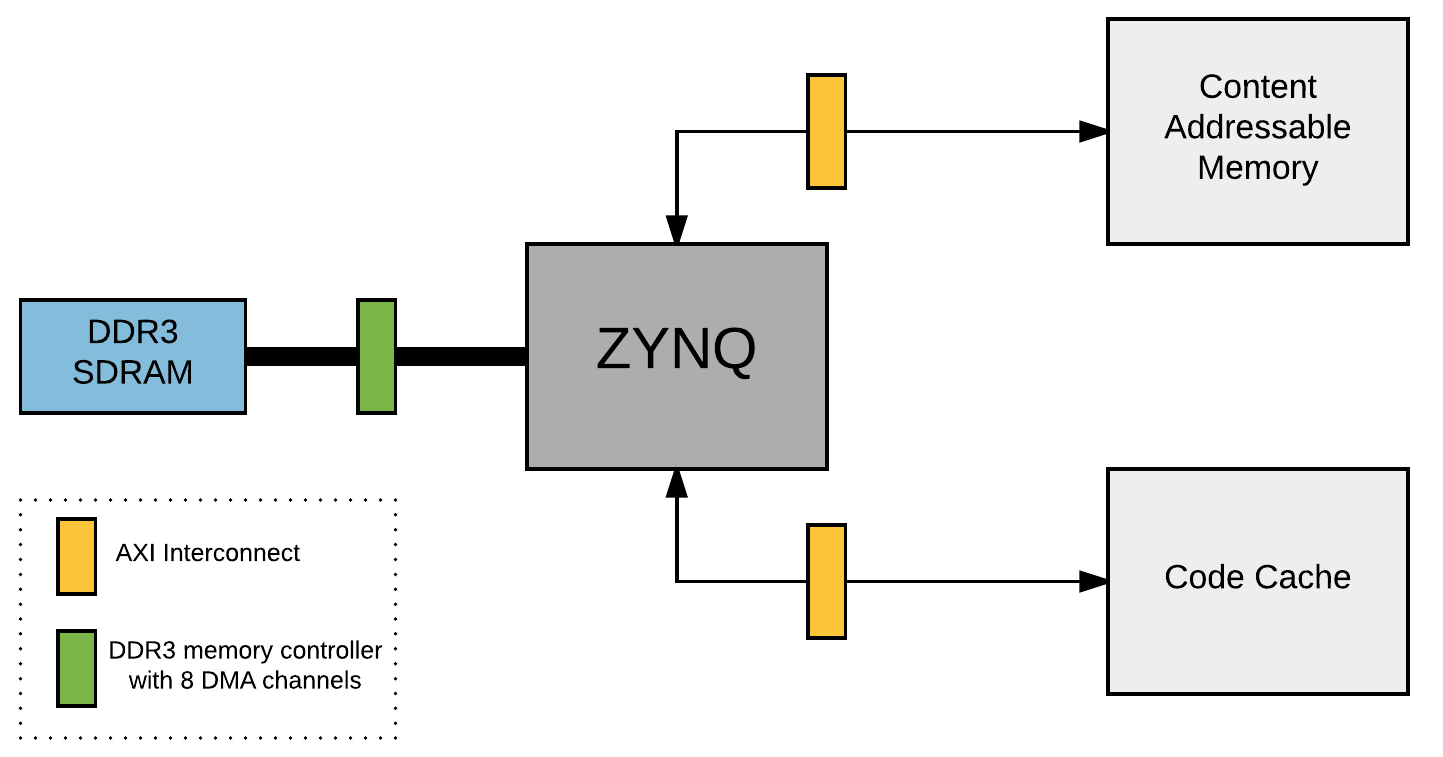
\includegraphics[scale = 0.2]{Images/DesignHw2.png}
	\caption{Content Addressable Memory hardware implementation with AXI Protocol}
	\label{fig:CAM_Hw}
\end{figure}

The second way is represented in the figure \ref{fig:CAM_Hw} and is probably the most efficient way is to implement only a Content Addressable Memory, that allows to know the address where a word is located. 

For this implementation we need a table that contains the initial PC of each translated basic block and the address where it is translated, it also stores the basic block size for management necessities.

\begin{figure} [H]
	\centering
	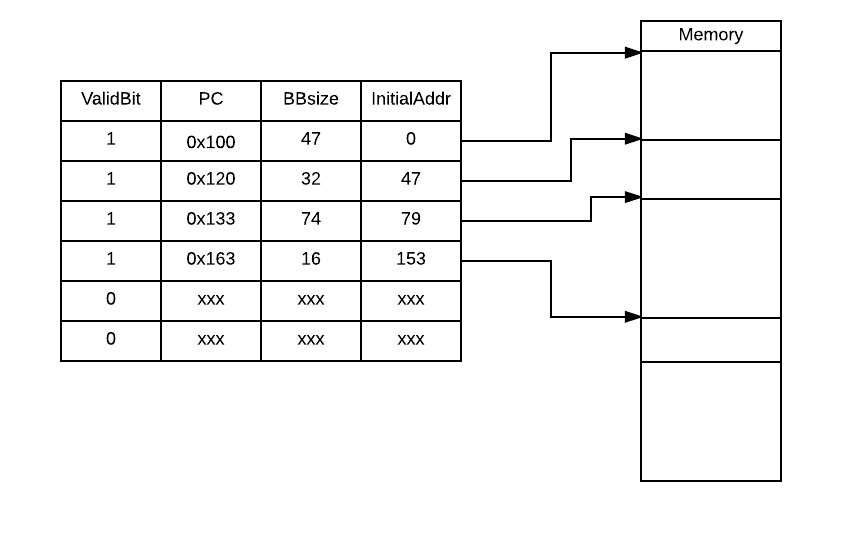
\includegraphics[scale = 0.35]{Images/CAM.png}
	\caption{Content Addressable Memory Table}
	\label{fig:CAM_table}
\end{figure}

This implementation also needs to respect the same interface, and so whenever we want to add a new tag, we first check if the number of basic blocks is maxed out, and if so we remove the oldest. Then we add an entree to the table saving the initial PC of the basic block, and the address corresponding to it that is the address of the previous basic block plus the previous basic block size.

\begin{figure} [h!]
	\centering
	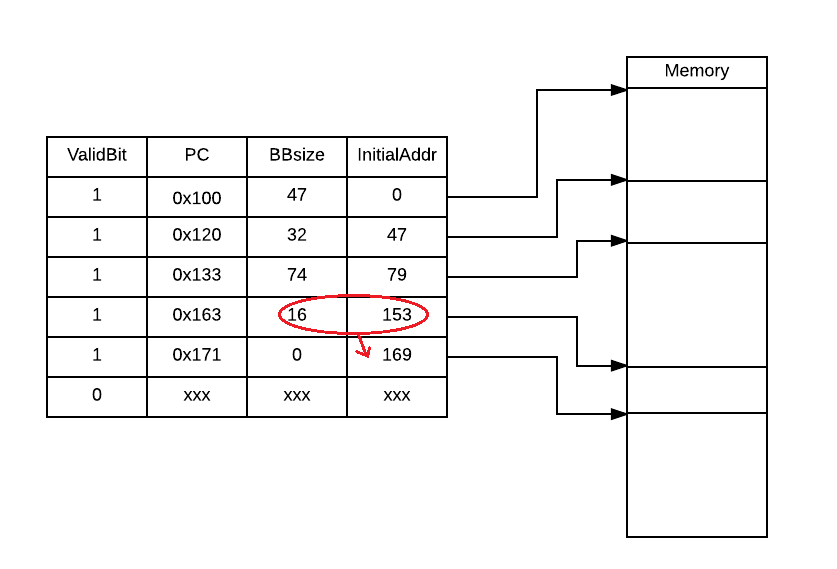
\includegraphics[scale = 0.35]{Images/CAM_new_BB.png}
	\caption{Content Addressable Memory Table: starting new basic block translation}
	\label{fig:CAMtableNewBB}
\end{figure}

To know if a basic block is translated we simply need to search the table for the initial PC and if there is a hit return the address where it is translated.
To perform the write operation, first it is necessary to check if there is room in the memory for the new instruction and if there isn't the oldest basic block must be removed. To do this it is not necessary to delete the basic block from memory, it's only needed to remove a line from the CAM as all management is done by the CAM, the data in memory will be overwritten. It's necessary to check if the basic block address plus the basic block size plus the new code size is bigger than the memory size. This means that we are in the end of the translation cache and the space that is available is in the beginning of the cache. When this happens we need to copy the basic block to the memory beginning and only then perform the write operation. To do this it's necessary to make room in the memory beginning to copy the entire basic block.


